\documentclass{bmvc2k}

%% Enter your paper number here for the review copy
%\bmvcreviewcopy{??}

%\usepackage[brazilian]{babel}
\usepackage[utf8]{inputenc}
\usepackage{bm}
\usepackage{amsmath}
\usepackage{tabularx}
\usepackage{siunitx}

\title{Projeto Demonstrativo 2}

% Enter the paper's authors in order
% \addauthor{Name}{email/homepage}{INSTITUTION_CODE}
\addauthor{Pedro Henrique Luz de Araujo}{pedrohluzaraujo@gmail.com}{1}
\addauthor{Rafael Barbosa de Sousa}{rafel.1940.b@gmail.com}{1}

% Enter the institutions
% \addinstitution{Name\\Address}
\addinstitution{
  Departamento de Ci\^encia da Comptuta\c{c}\~ao\\
  Universidade de Bras\'{\i}lia\\
  Campus Darcy Ribeiro, Asa Norte\\
  Bras\'{\i}lia-DF, CEP 70910-900, Brazil,  
}

\runninghead{Luz de Araujo, P.H.; de Sousa, R. B.}{PD2 -- \today}

% Any macro definitions you would like to include
% These are not defined in the style file, because they don't begin
% with \bmva, so they might conflict with the user's own macros.
% The \bmvaOneDot macro adds a full stop unless there is one in the
% text already.
\def\eg{\emph{e.g}\bmvaOneDot}
\def\ie{\emph{i.e}\bmvaOneDot}
\def\Eg{\emph{E.g}\bmvaOneDot}
\def\etal{\emph{et al}\bmvaOneDot}
\newcommand{\norm}[1]{\left\lVert#1\right\rVert}
\newcommand\blfootnote[1]{%
  \begingroup
  \renewcommand\thefootnote{}\footnote{#1}%
  \addtocounter{footnote}{-1}%
  \endgroup
}


%-------------------------------------------------------------------------
% Document starts here
\begin{document}
\begin{NoHyper}
\maketitle
\end{NoHyper}

\begin{abstract}
O presente Projeto Demonstrativo visa a implementar um programa capaz de medir o tamanho de objetos a partir das dimensões correspondentes em uma imagem. Para tanto, calibra-se a câmera usada para captura das imagens, a fim de conhecer os parâmetros da transformação do mundo tridimensional para o plano da imagem, que podem ser intrínsecos ou extrínsecos. Comparamos duas formas de obtenção dos extrínsecos - estimando-os juntamente com os intrínsecos, ou a partir dos intrínsecos e novas imagens - a três distâncias diferentes em cada caso. Obtivemos medidas que se aproximam do esperado, mas concluímos que a técnica pode não servir bem para aplicações que necessitam medidas mais precisas.\footnote{Pedro contribuiu com o código principal do projeto e com medidas próprias. Rafael contribuiu com o \textit{script calibrate.py}, com medidas próprias e com a comparação entre os dois cenários de cálculo de parâmetros extrínsecos.}
\end{abstract}

%-------------------------------------------------------------------------
\section{Introdução}
\label{sec:intro}

O processo de formação de imagens pelas câmeras pode ser entendido como a projeção de uma representação bidimensional
de um mundo tridimensional. Tal transformação é um processo que pode ser modelado por uma projeção central na qual um raio de um ponto do espaço tridimensional passa por um centro de projeção e intersecciona um ponto no plano da imagem~\cite{Hartley:2003:MVG:861369}. Aprender o mapeamento de pontos do mundo para pontos da imagem é central em aplicações como: remoção de distorções; estimação de estrutura tridimensional e medidas de objetos; e estimação de profundidade.

Tal mapeamento pode ser expresso da seguinte forma:

\begin{equation}
    \label{proj}
    \lambda
    \begin{bmatrix}
    u \\
    v \\
    1 \\
    \end{bmatrix}
    =
    \mathbf{P}_{3x4}
    \begin{bmatrix}
    X \\
    Y \\
    Z \\
    1
    \end{bmatrix}\,,
\end{equation}
em que $(u, v, 1)$ e $(X, Y, Z, 1)$ são as coordenadas homogêneas do ponto na imagem e no mundo, respectivamente, e $\mathbf{P}_3x4$ é a matriz que realiza a transformação, a qual depende tanto de características da câmera (parâmetros intrínsecos) quanto das coordenadas adotadas (parâmetros extrínsecos).

Segundo~\cite{Forsyth:2002:CVM:580035}, existem cinco parâmetros intrínsecos: $f_x$ e $f_y$ são as distâncias focais expressas em pixeis (exige-se dois parâmetros para o caso de pixeis não quadrados); $c_x$ e $c_y$ definem as coordenadas do centro da imagem; e $\theta$ indica o ângulo entre os dois eixos da imagem. Esse último parâmetro é igual a zero quando tal ângulo é reto, aproximação usada por nós.


Uma vez que os parâmetros intrínsecos adotam coordenadas centradas na câmera, surge a necessidade de deslocar a transformação caso deseje-se outro sistema de coordenadas. Os parâmetros extrínsecos são responsáveis por isso, descrevendo uma matriz de rotação $\mathbf{R}_{3x3}$ e um vetor de translação $\bm{t}$. Portanto, a equação \ref{proj} pode ser reescrita como:

\begin{equation}
    \label{world2cam}
    \lambda
    \begin{bmatrix}
    u \\
    v \\
    1 \\
    \end{bmatrix}
    =
    \begin{bmatrix}
    f_x & 0 & c_x \\
    0 & f_y & c_y \\
    0 & 0 & 1
    \end{bmatrix}
    \begin{bmatrix}
    r_{11} & r_{12} & r_{13} & t_1  \\
    r_{21} & r_{22} & r_{23} & t_2  \\
    r_{31} & r_{32} & r_{33} & t_3
    \end{bmatrix}
    \begin{bmatrix}
    X \\
    Y \\
    Z \\
    1
    \end{bmatrix}\,.
\end{equation}


Tal modelo é acourado apenas para uma câmera ideal, em que o ponto no mundo e na imagem e o centro óptico são co-lineares. Entretanto, câmeras reais apresentam distorções, entre elas, a distorção radial. Para remediar essa situação, é preciso corrigir as medidas da imagem para aquelas que seriam obtidas por uma câmera ideal (perfeitamente linear)~\cite{Hartley:2003:MVG:861369}. A distorção radial pode ser modelada por um polinômio de grau baixo~\cite{Forsyth:2002:CVM:580035}, cujos coeficientes são denominados coeficientes de distorção.


A calibração da câmera consiste em calcular todos esses parâmetros. Podemos fazê-lo a partir de correspondências entre pontos no mundo real e suas projeções no mundo da imagem. Com isso, obtemos equações que relacionam tais pontos, em que os parâmetros que queremos calcular são as incógnitas. A partir daí basta resolver as equações empregando métodos de otimização e técnicas de álgebra linear.

\section{Metodologia}
\label{sec:met}
\subsection{Ferramentas}
Usamos a biblioteca OpenCV~\cite{opencv_library}, versão 3.3.0, para a captura de video de \textit{webcam} e para obter os parâmetros da câmera. Para realizar operações sobre as matrizes de imagens, utilizamos a biblioteca de computação numérica em Python, NumPy. Usamos ainda, como linguagem, Python 3.5.2, e o gerenciador de bibliotecas Anaconda 3.

\subsection{Requisito 1}
O requisito 1 trata da obtenção da distância entre dois pixeis de uma imagem. A partir de funções da biblioteca OpenCV, é exibida na tela do usuário a captura da \textit{webcam}. O usuário tem a faculdade de clicar em dois pontos quaisquer da captura, momento em que uma linha vermelha é desenhada no \textit{frame} e são exibidos no terminal as coordenadas de ambos os pontos, além da distância entre eles.

A distância medida é a distância euclideana em duas dimensões, isto é, a norma do vetor de diferença entre os dois pontos. Sejam $\bm{u}=(x_i, y_i)$ e $\bm{v}=(x_f, y_f)$ os pontos inicial e final a serem medidos. Então:
\begin{equation}
    d=\sqrt{(x_f-x_i)^2 + (y_f-y_i)^2} = \norm{\bm{v}-\bm{u}}\,,
\end{equation}
em que d é a distância entre os dois pontos. A norma entre os dois vetores pode ser obtida por meio da biblioteca de álgebra linear do NumPy.

\subsection{Requisito 2}
O objetivo do requisito 2 é obter os parâmetros da matriz intrínseca de uma câmera além dos coeficientes de distorção. Para tanto, utilizou-se uma padrão de calibração como mostrado na figura \ref{chess}. Podemos encarar o tabuleiro de xadrez como uma rede de 48 pontos, localizados nas esquinas dos quadrados internos do tabuleiro. Assumindo o lado do quadrado como a unidade fundamental, possuímos, assim a coordenada dos 48 pontos, considerando a origem como a primeira intersecção entre quatro quadrados (a do canto superior esquerdo). Para estimar os parâmetros intrínsecos precisamos, além das coordenadas dos objetos, das coordenadas correspondentes na imagem.

\begin{figure}[htb] 
\centering
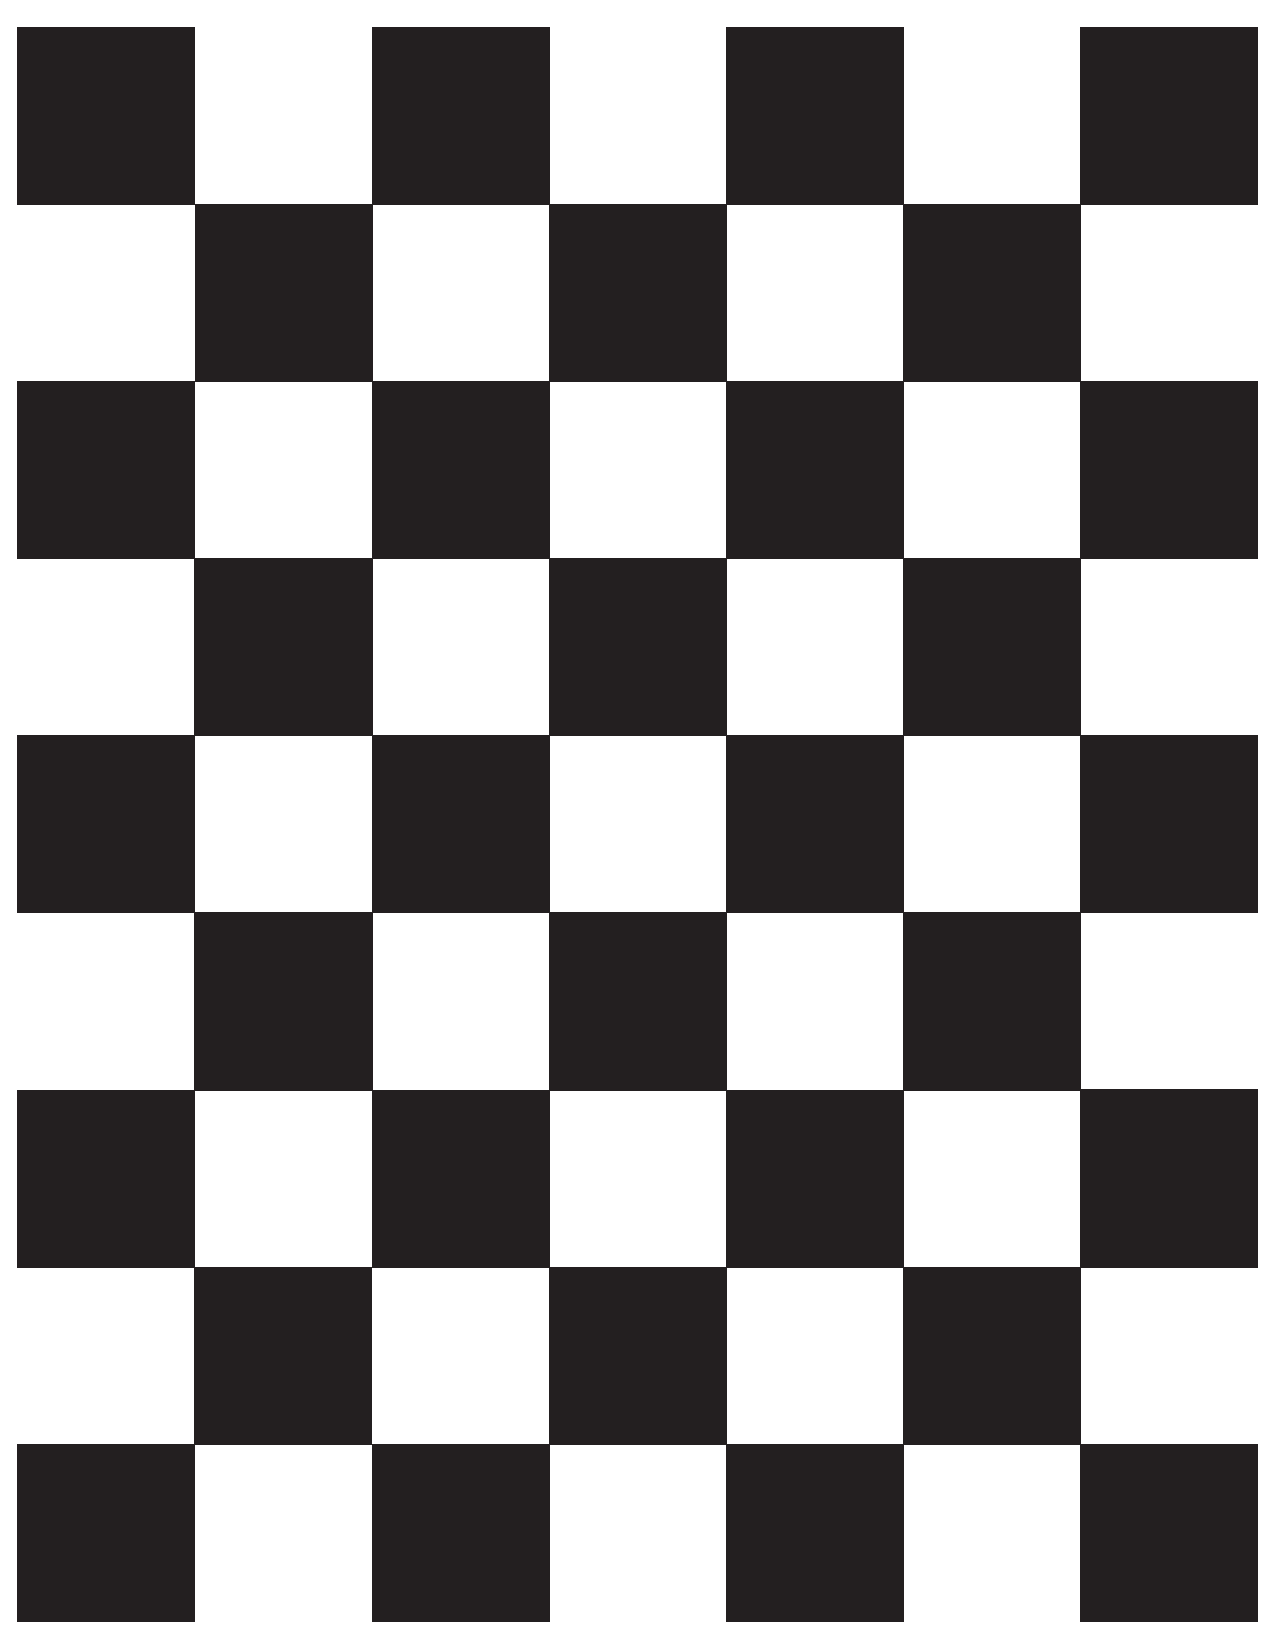
\includegraphics[width=0.2\textwidth, angle=90]{figs/pattern.pdf}
\caption{Padrão usado para calibração \label{chess}}
\end{figure}

Para tanto, utilizamos a biblioteca OpenCV para obter automaticamente as coordenadas das esquinas do tabuleiro. Assim, de posse das coordenadas de pontos no mundo real e sua correspondência na imagem, a biblioteca OpenCV pode ser utilizada para estimar os parâmetros intrínsecos. O algoritmo utilizado é baseado em \cite{zhang2000flexible} e \cite{bouguet2002camera} e consiste em três etapas:
inicialização dos valores dos parâmetros intrínsecos e dos coeficientes de distorção; estimativa da pose da câmera a partir desses valores iniciais; e minimização do erro de re-projeção, isto é, a soma das distâncias quadradas entre os pontos da imagem e os pontos projetadas a partir das estimativas dos parâmetros.

Para a calibração, capturamos cinco imagens do tabuleiro sob diferentes posições. Tal procedimento foi repetido cinco vezes de modo a obter a média e o desvio padrão da matriz de parâmetros intrínsecos e dos coeficientes de distorção.

De posse dessas medidas, foi possível reverter a distorção gerada pela câmera a cada frame capturado pela \textit{webcam}, de modo a possibilitar de medição de distâncias em pixeis tanto na captura \textit{raw}, ou distorcida, quanto na captura \textit{undistorted}, ou corrigida. A correção da distorção é simples uma vez que temos os coeficientes de distorção~\cite{zhang2000flexible}:


\begin{subequations}
    \begin{align}
    \widetilde{x}&=x+x[k_1(x^2+y^2] + k_2(x^2+y^2)^2] \\
    \widetilde{y}&=y+y[k_1(x^2+y^2] + k_2(x^2+y^2)^2]\,,
    \end{align}
\end{subequations}
em que $\widetilde{x}$ e $\widetilde{y}$ são as coordenadas após correção e $k_1$ e $k_2$ são os coeficientes de distorção.

\subsection{Requisito 3}
\label{met3}
O requisito 3 requer o cálculo dos parâmetros extrínsecos da câmera a partir de três distâncias distintas: $d_{min}$, a menor distância possível em que é possível observar os 48 pontos do padrão de calibração; $d_{max}$, a maior distância que permitia a captura dos pontos pelo OpenCV; e $d_{med}$, uma distância intermediária. Realizamos a medida dos parâmetros extrínsecos de duas maneiras diferentes.

Na primeiro cenário, que denominamos \textit{bônus}, os parâmetros extrínsecos foram obtidos juntamente com os intrínsecos, por meio do algoritmo mencionado na subseção anterior.

No segundo cenário, o \textit{regular}, os extrínsecos foram obtidos a partir da matriz de intrínsecos e dos coeficientes de distorção calculados no requisito 2. Primeiramente, medimos o lado do quadrado do padrão de calibração e, adotando o primeiro ponto como origem do mundo e  $z=0$ para todos os pontos do padrão, armazenamos as coordenadas reais de cada um dos 48 pontos em milímetros. 

Em seguida, posicionamos a origem padrão de calibração à correspondente distância ao centro da câmera e capturamos uma imagem. Assim, a partir dos parâmetros intrínsecos, dos coeficientes de distorção, das coordenadas reais dos pontos, e das coordenadas correspondentes na imagem obtidas pelo OpenCV, calculamos os parâmetros extrínsecos por meio da função solvePnP, da mesma  biblioteca. Esse procedimento foi feito três vezes para cada uma das distâncias, sendo calculado a média e o desvio padrão dos parâmetros extrínsecos de cada distância.

Destacamos que os parâmetros são obtidos na forma de um vetor de rotação $\bm{r}$  e um vetor de translação $\bm{t}$. Para obter a matriz de rotação $\mathbf{R}$ basta aplicar o algoritmo Rodrigues em $\bm{r}$. A matriz de extrínsecos, então, é a concatenação de $\mathbf{R}$ e $\bm{t}$.

\subsection{Requisito 4}
O requisito 4 trata do uso da calibração para obtenção de medidas reais de objetos. Uma vez que as matrizes de calibração da câmera transformam coordenadas do mundo em coordenadas da imagem, podemos gerar uma transformação inversa para, a partir de coordenadas em pixeis da imagem, obter medidas reais de objetos. Dada a equação \ref{world2cam}, podemos multiplicar a matriz de parâmetros intrínsecos pela de extrínsecos:
\begin{equation}
    \lambda
    \begin{bmatrix}
    u \\
    v \\
    1 \\
    \end{bmatrix}
    =
    \begin{bmatrix}
    a_{11} & a_{12} & a_{13} & a_{14}  \\
    a_{21} & a_{22} & a_{23} & a_{24}  \\
    a_{31} & a_{32} & a_{33} & a_{34}
    \end{bmatrix}
    \begin{bmatrix}
    X \\
    Y \\
    Z \\
    1
    \end{bmatrix}\,.
\end{equation}
Mas $Z=0$, já que medimos apenas objetos localizados no plano do padrão de calibração, de modo que podemos retirar a terceira coluna da matriz \textbf{A}:
\begin{equation}
    \lambda
    \begin{bmatrix}
    u \\
    v \\
    1 \\
    \end{bmatrix}
    =
    \begin{bmatrix}
    a_{11} & a_{12}  & a_{14}  \\
    a_{21} & a_{22}  & a_{24}  \\
    a_{31} & a_{32}  & a_{34}
    \end{bmatrix}
    \begin{bmatrix}
    X \\
    Y \\
    1
    \end{bmatrix}\,.
\end{equation}
Assim, obtemos a matriz inversa $\textbf{A}^{-1}$:
\begin{equation}
    \begin{bmatrix}
    X \\
    Y \\
    1
    \end{bmatrix}
    =
    \lambda
    \begin{bmatrix}
    a_{11} & a_{12}  & a_{14}  \\
    a_{21} & a_{22}  & a_{24}  \\
    a_{31} & a_{32}  & a_{34}
    \end{bmatrix}^{-1}
    \begin{bmatrix}
    u \\
    v \\
    1 \\
    \end{bmatrix}\,,
\end{equation}
que é a transformação que usamos para obter as coordenadas reais de objetos.

Por meio dessa transformação, medimos a dimensão real de objetos a partir da correspondente medida na imagem do objeto. Foram medidos dois objetos diferentes: um livro (figura \ref{livro}) e um porta-fita (figura \ref{fita}). Os objetos foram medidos nas três distâncias mencionadas no requisito 3. Além disso, realizaram-se medidas nas janelas \textit{raw} e \textit{undistorted}, com o objeto posicionado no centro e na periferia da janela. Em cada uma dessas situações foram realizadas duas medidas, obtendo-se assim a média e o desvio padrão da dimensão do objeto. Por fim, tal procedimento foi realizado com duas câmeras: a de Pedro e a de Rafael. Neste último caso, mediu-se ainda com parâmetros extrínsecos do cenário \textit{regular} e \textit{bonus}.

\begin{figure}
\centering
\begin{minipage}[t]{0.45\textwidth}
  \centering
  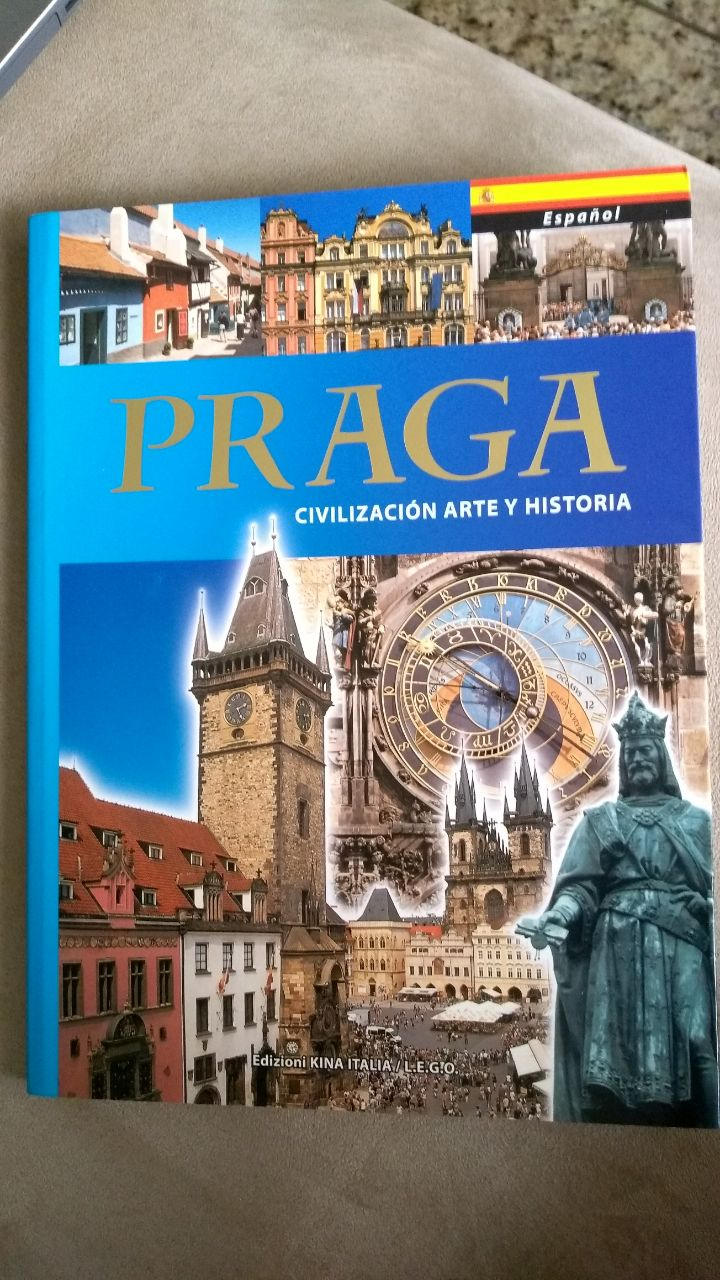
\includegraphics[height=\linewidth, angle=90]{figs/objeto_pedro.jpg}
  \caption{Livro com largura medida por Pedro.}
  \label{livro}
\end{minipage}\hfill
\begin{minipage}[t]{0.45\textwidth}
  \centering
  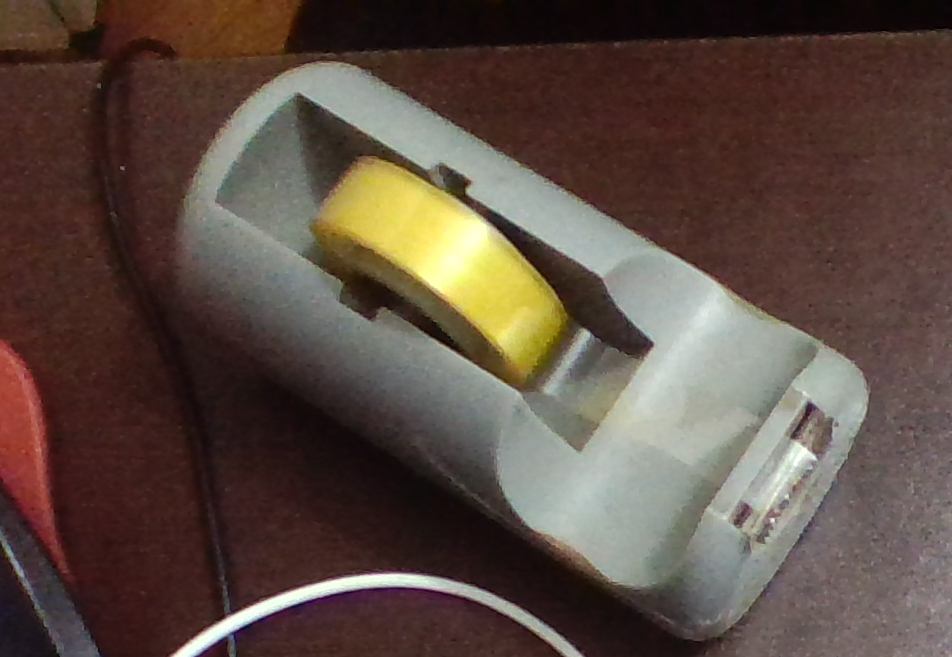
\includegraphics[width=\linewidth]{figs/objeto_rafael.png}
  \caption{Porta-fita com comprimento medido por Rafael.}
  \label{fita}
\end{minipage}
\end{figure}


\section{Resultados}
\label{sec:res}
\subsection{Requisito 1}
A figura \ref{fig:requisito 1} apresenta o resultado de uma medição de distância entre dois pontos do plano da imagem em pixeis. É possível perceber o correto cômputo das coordenadas dos pixeis em questão e da distância euclidiana entre eles.

\begin{figure}[hbt]
  \centering
  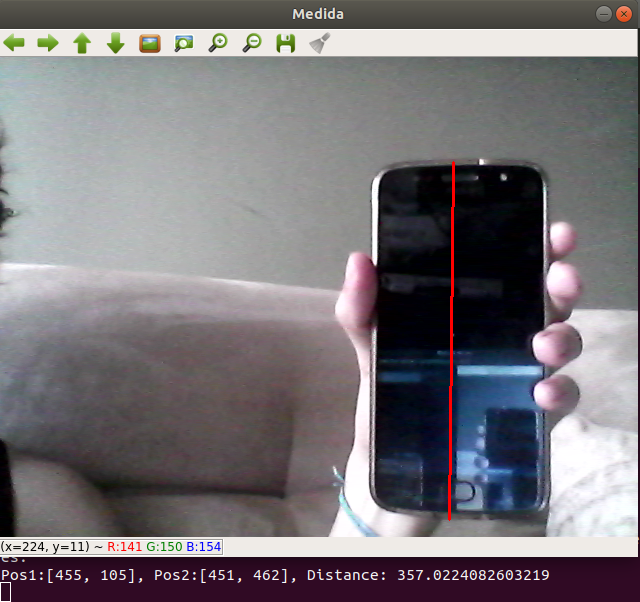
\includegraphics[width=0.3\textwidth]{figs/requisito1.png}
  \caption{Exemplo de medição do requisito 1.}
  \label{fig:requisito 1}
\end{figure}


\subsection{Requisito 2}
O requisito 2 gerou parâmetros intrínsecos e coeficientes de distorção para as câmeras de ambos autores. As tabelas \ref{table:int_pedro} e \ref{table:int_rafael} apresentam os valores encontrados para os parâmetros intrínsecos, com o desvio padrão como margem de erro.\footnote{Os coeficientes de distorção de cada câmera podem ser encontrados na pasta \textit{xmls} do projeto. Optamos por não os apresentar aqui por possuírem baixa interpretabilidade e não acrescentarem às análises que desejamos realizar.} A figura \ref{fig:requisito 2} compara a exibição das janelas \textit{raw} e \textit{undistorted}.

\begin{table}[hbt]
\begin{minipage}{.5\linewidth}
 \small
\caption{Parâmetros da câmera de Pedro.}
\label{table:int_pedro}
\centering
\begin{tabular}{| c | c |}
\hline
Parâmetro & Valor \\
\hline
$f_x$  & \num{7.8e+2} $\pm$  \num{0.1e+2} \\
$f_y$  & \num{7.8e+2} $\pm$  \num{0.1e+2} \\
$c_x$  & \num{3.7e+2} $\pm$  \num{0.3e+2} \\
$c_y$  & \num{2.30e+2} $\pm$  \num{0.08e+2} \\
\hline
\end{tabular}
\end{minipage}%
\begin{minipage}{.5\linewidth}
 \small
\caption{Parâmetros da câmera de Rafael.}
\label{table:int_rafael}
\centering
\begin{tabular}{| c | c |}
\hline
Parâmetro & Valor \\
\hline
$f_x$  & \num{1.53e+3} $\pm$  \num{0.04e+3} \\
$f_y$  & \num{1.54e+3} $\pm$  \num{0.04e+3} \\
$c_x$  & \num{9.38e+2} $\pm$  \num{0.04e+2} \\
$c_y$  & \num{5.9e+2} $\pm$  \num{0.3e+2} \\
\hline
\end{tabular}
\end{minipage}
\end{table}

\begin{figure}[htb]
  \centering
  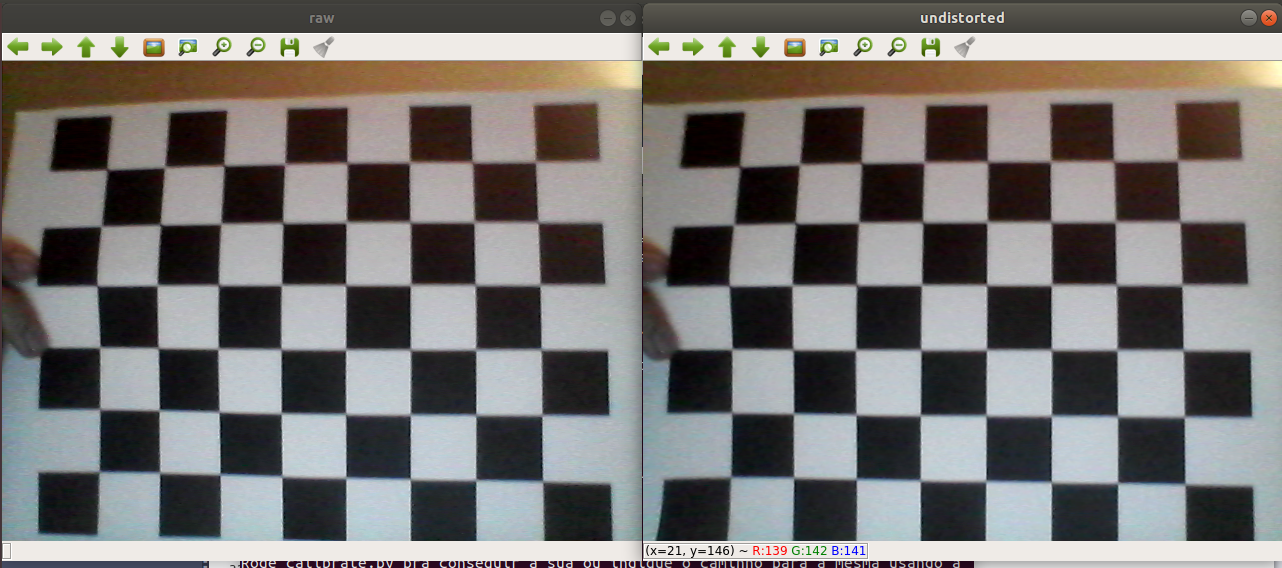
\includegraphics[width=0.5\textwidth]{figs/rawXcor.png}
  \caption{Comparação entre imagem bruta (à esquerda) e com distorção corrigida.}
  \label{fig:requisito 2}
\end{figure}

\subsection{Requisito 3}
Obtivemos vetores de rotação e de translação para as câmeras de Pedro e de Rafael, sendo que neste caso, os vetores foram calculados de duas formas diferentes, como descrito na subseção \ref{met3}.\footnote{Todas os vetores obtidos estão presentes no diretório ``xmls'' do projeto.} A tabela \ref{table:norm} compara a distância real entre a câmera e a origem com a norma do vetor de translação obtido para cada caso.\footnote{O erro da norma foi obtido pela propagação dos desvios padrão das medidas do vetor em questão. O erro relativo trata do desvio percentual entre a norma calculada e a distância real.}

\begin{table}[htb]
 \small
\caption{Comparação entre a distância $d$ real e a norma da translação $\norm{\bm{t}}$ calculada.}
\label{table:norm}
\centering
\begin{tabular}{| c | c | c | c |}
\hline
& $d$ (m) & $\norm{\bm{t}}$ (m) & Erro relativo\\
\hline
$d_{min}$ Pedro & $0.402$  & $0.387 \pm 0.008$ & $3.73\%$ \\
$d_{med}$ Pedro & $1.030$  & $0.99 \pm 0.05$ & $3.88\%$ \\
$d_{max}$ Pedro & $1.740$  & $1.79 \pm 0.02$ & $2.79\%$ \\
$d_{min}$ Rafael & $0.290$  & $0.43 \pm 0.02$ & $48.27\%$ \\
$d_{med}$ Rafael & $1.205$  & $1.28 \pm 0.01$ & $6.22\%$ \\
$d_{max}$ Rafael & $2.700$  & $2.7 \pm 0.3$ & $0$ \\
$d_{min}$ Bônus & $0.290$  & $0.01088 \pm 0.00009$ & $96.25\%$ \\
$d_{med}$ Bônus & $1.205$  & $0.0726 \pm 0.0003$ & $93.98\%$ \\
$d_{min}$ Bônus & $2.700$  & $0.085 \pm 0.001$ & $96.85\%$ \\
\hline
\end{tabular}
\end{table}

\subsection{Requisito 4}
As tabelas \ref{table:medidasP} e \ref{table:medidasR} demonstram as diversas medições realizadas para o requisito 4 em cada cenário. $l_{real}$ representa a medida real do objeto em questão, $l_{raw}$ a medida na janela \textit{raw}, $l_{undistorted}$ a medida na janela \textit{undistorted}, $l_{center}$ medida realizada no centro da tela e $l_{perifery}$ medida realizada nos cantos da tela. Todas as distâncias estão em metros.

\begin{table}[htb]
 \footnotesize
\caption{Medidas encontradas a partir de imagens com $l_{real}=0.196m$ (livro).}
\label{table:medidasP}
\centering
\begin{tabular}{| c | c | c | c |}
\hline
 & \multicolumn{3}{|c|}{Pedro} \\
\hline
Distância & $d_{min}$ & $d_{med}$ & $d_{max}$\\
\hline
$\norm{\bm{t}_{real}}$ & $0.402$ & $1.030$ & $1.740$ \\
$\norm{\bm{t}}$ & $0.387 \pm 0.008$ & $0.99 \pm 0.05$ & $1.79 \pm 0.02$ \\
\hline
$\norm{\bm{l}}_{raw, center}$ & $0.161 \pm 0.001$ & $0.17 \pm 0.01$ & $1.56 \pm 0.04$ \\
$\norm{\bm{l}}_{raw, perifery}$ & $0.167 \pm 0.002$ & $0.155 \pm 0.005$ & $0.170 \pm 0.004$ \\
$\norm{\bm{l}}_{undistorted, center}$ &$0.163 \pm 0.001$ & $0.172
\pm 0.006$ & $0.168 \pm 0.04$ \\
$\norm{\bm{l}}_{undistorted, perifery}$ & $0.168 \pm 0.003$ & $0.167 \pm 0.001$ & $0.167 \pm 0.001$ \\
\hline
\end{tabular}
\end{table}

\begin{table}[htb]
 \tiny
\caption{Medidas encontradas a partir de imagens com $l_{real}=0.105m$ (porta-fita).}
\label{table:medidasR}
\centering
\tabcolsep=0.11cm
\begin{tabular}{| c | c | c | c | c | c | c |}
\hline
 & \multicolumn{3}{|c|}{Rafael} & \multicolumn{3}{|c|}{\textit{Bonus}} \\
\hline
 Distância & $d_{min}$ & $d_{med}$ & $d_{max}$ & $d_{min}$ & $d_{med}$ & $d_{max}$\\
 \hline
$\norm{\bm{t}_{real}}$ & $0.290$ & $1.205$ & $2.700$  & $0.290$ & $1.205$ & $2.700$ \\
$\norm{\bm{t}}$ & $0.43 \pm 0.02$ & $1.28 \pm 0.01$ & $2.7 \pm 0.3$ & $0.01088 \pm 0.00009$ & $0.0726 \pm 0.0003$ & $0.085 \pm 0.001$ \\
\hline
$\norm{\bm{l}}_{raw, center}$ & $0.135 \pm 0.001$ & $0.106 \pm 0.002$ & $0.125 \pm 0.001$ & $0.036 \pm 0.001$ & $0.062 \pm 0.001$ & $0.037 \pm 0.001$ \\
$\norm{\bm{l}}_{raw, perifery}$ & $0.156 \pm 0.005$ & $0.112 \pm 0.001$ & $0.126 \pm 0.005$ & $0.037 \pm 0.003$ & $0.072 \pm 0.001$ & $0.046 \pm 0.001$ \\
$\norm{\bm{l}}_{undistorted, center}$ &$0.139 \pm 0.006$ & $0.098
\pm 0.004$ & $0.121 \pm 0.005$ &$0.037 \pm 0.002$ & $0.060
\pm 0.001$ & $0.038 \pm 0.002$ \\
$\norm{\bm{l}}_{undistorted, perifery}$ & $0.137 \pm 0.001$ & $0.104 \pm 0.001$ & $0.122 \pm 0.004$ & $0.031 \pm 0.001$ & $0.060 \pm 0.001$ & $0.047 \pm 0.003$ \\
\hline
\end{tabular}
\end{table}


\section{Discussão e Conclusões}
\label{sec:disc}
Primeiramente discutiremos o cenário \textit{regular}, tanto de Pedro e Rafael, para em seguida tecer considerações sobre o cenário \textit{bonus}.

Percebeu-se que a norma do vetor de translação se aproxima mais
do valor real na distância $d_{max}$, apresentado o pior valor em $d_{med}$. Ainda, nota-se dos dados que as aproximações são boas, com erros inferiores a $6.22\%$, com a exceção de um \textit{outlier} em $d_{min}$ de Rafael, possivelmente por algum problema no momento de captura das imagens para o cálculo dos parâmetros externos.

As medidas do objeto de Pedro apresentam valores semelhantes em todas as três distâncias e se aproximam da medida real, sendo que os valores que mais fogem da média são aqueles calculados na periferia da imagem distorcida, como esperado. No caso de Rafael, os valores se aproximam bem do esperado nas distâncias $d_{med}$ e $d_{max}$, apresentando um erro maior em $d_{min}$. Isso possivelemente está relacionado pelo erro da norma do vetor de translação nessa distância, como mencionamos no parágrafo anterior.

Quanto ao cenário \textit{bonus}, nota-se que os valores da norma da translação e das medidas do objeto são muito inferiores ao esperado. Isso pode ser explicado pelo fato de não serem informadas as medidas do quadrado do padrão de calibração no momento da obtenção dos parâmetros, de modo que os extrínsecos são obtidos em alguma unidade de medida arbitrária. Dito isso, é possível analisar que os tamanhos encontrados são compatíveis nos casos $d_{min}$ e $d_{max}$. Infelizmente o fato das medidas do cenário \textit{bonus} estarem em unidades arbitrárias dificulta comparações com o cenário \textit{regular}.

O presente trabalho demonstrou que a calibragem de câmeras permite a obtenção de medidas aproximadas do mundo real a partir de uma única imagem. Embora tais medidas se aproximem do valor real, o erro encontrado impossibilitaria o uso da técnica para aplicações que exigem precisão na casa dos centímetros. Observou-se, também, a possibilidade de obtenção dos parâmetros intrínsecos e extrínsecos de uma só vez. Nesse caso, quando não fornecemos ao algoritmo as medidas dos quadrados do plano de calibração, verificamos que ele retorna parâmetros em alguma unidade arbitrária. 

O uso de técnicas \textit{stereo}, com mais de uma câmera, possivelmente forneceria medidas mais precisas. Alternativamente, um ambiente mais propício para calibração, com iluminação, suporte, trilhos e outro utensílios também forneceria medidas mais confiáveis.



\clearpage
\bibliography{refs}
\end{document}
